\chapter{绪论}\label{sec:introduction}

本章阐述了此次毕业设计的背景,目前行业内的研究现状,此次毕业设计的研究问题以及此设计的主要工作与创新点等内容。

\section{研究背景}

近年来 随着诸如 4G、高速宽带网络以及智能手机技术的飞速进步。人们的休闲娱乐重心逐渐从文字与图片相关内容转移到了短视频与直播应用上。市场上也涌现出了一系列的短视频应用软件。本毕业设计课题将完成短视频应用开发的整个流程。

目前短视频应用已经成为互联网产业链中一个重要的流量入口。截止 2018 年 12 月,在线视频行业月独立设备数达 10.17 亿,同比增长 1.7\%,其中短视频行业月独立设备数达 7.34 亿台,同比增长率为 58.7\%,用户短视频应用使用时长达到了总上网时长的 8.2\%\cite{中国互联网络信息中心2018第}。在智能手机已经普及的今天,短视频相关应用已经爆发出了强大的活力,具有相当高的市场价值。所以进行短视频应用开发对于我们认识短视频应用相关技术以及商业模式具有非常大的帮助作用。

短视频应用主要功能为接受用户上传的视频并对其进行一系列的处理,如:转码、压缩、合并背景音乐以及提取关键帧等操作。服务器在进行视频相关操作时所承受的压力较大,对于多用户同时上传视频的情景需要设计出一种合理的视频操作解决方案并进行一系列优化。如何合理地处理此种情景也是十分重要的。此外,视频的长度、清晰度、码率、上传的格式也会对服务器的视频操作压力产生影响,因此,本次毕业设计需在视频上传前对视频进行预处理。

当网络应用的用户数较大、同时访问人数较多时,应用系统的瓶颈通常位于服务器的 I/O 输入输出、数据库的操作以及服务器的带宽上,此时,单纯的增加服务器的数量往往不能有效地解决问题\cite{rosenfeld2002information}。因此,合理设计应用系统架构、合理地进行技术选型是非常有用的,有必要对各类型应用架构进行深入地调查、分析与研究。

\section{研究现状}
本节引入了与本设计紧密相关的部分内容:Java Web 技术、数据库技术、视频编码技术以及微信小程序技术。

\subsection{Java Web 技术}

Java Web 技术即使用 Java 语言开发运行在 JVM(Java 虚拟机) 上的网络应用程序的技术。其主要任务是开发出具有合理、高效、低耦合、高内聚、较少错误和较好的可扩展性等优点的应用\cite{arnold2005java}。Java Web 开发需基于 Java 官方给出的 Java EE 规范,且网络应用需运行在 Java 容器或 Java 网络服务器中。随着网络技术以及网络应用的发展,Sun 公司研发了 Servlet 技术。Servlet 是一个能够处理 HTTP 请求的 Java 程序。随着 Servlet 的几轮技术迭代,Sun 公司发布了基于 Java 2 平台的 Java 企业版。由此揭开了 Java 用于网络应用开发的大幕。现在,行业内一般使用某种 Java Web 框架作为基础进行开发,搭配 MVC 技术、ORM 技术以及 Web 服务器进行相关功能的实现。常用的框架有 EJB 框架以及 Spring 框架\cite{williams2014professional}。

EJB 即 Enterprise Java Bean 是一个企业级的 Java 框架,内置了 JBOSS 服务器。图\ref{fig:ejb} 是 EJB 框架的架构图,EJB 框架提供了分布式应用功能,即你可以将一个应用分散到多个服务器上,由多个 Java 虚拟机一同运行\cite{johnson2004expert}。此外 EJB 还提供了组件化支持与持久化管理功能。EJB 技术可以有效地提高 Java 企业级应用开发的效率,但与此同时,EJB 也产生了许多负面影响,如:EJB 使得应用系统更难测试、使应用系统更难部署、破坏了面向对象准则等。因此需要合理地抉择是否使用 EJB。需要使用 EJB 的情景有:应用的部分组件需要被远程访问的情景以及需要对应用进行分布式部署的情景。


% \begin{tikzpicture}
%     % [L1Node/.style={circle,   draw=blue!50, fill=blue!20, very thick, minimum size=10mm},
%     % L2Node/.style={rectangle,draw=green!50,fill=green!20,very thick, minimum size=10mm}]
%     [
%         L1Node/.style={rectangle,draw=green!50,fill=green!20,very thick, minimum size=10mm},
%         Tag/.style={rectangle}
%     ]

%     \draw (0,0) rectangle (10, 15);
%     \node[Tag] (tag1) at (5, 15){EJB 架构图};
%     \node[L1Node] (n1) at (2, 2){JSP};

% \end{tikzpicture}

\begin{figure}[!ht]
    \centering
    %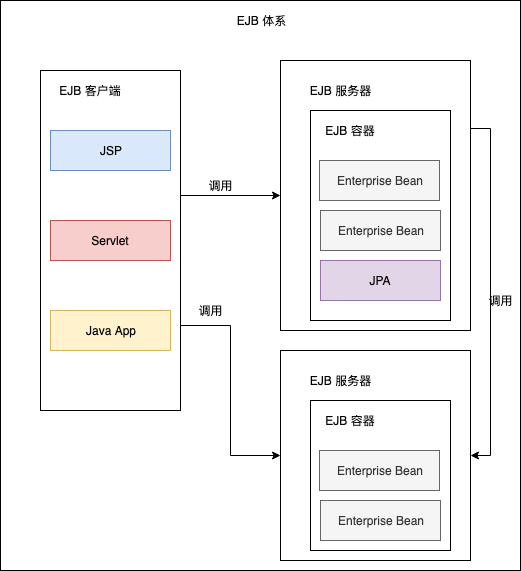
\includegraphics[width=0.7\textwidth]{EJB.png}
    \begin{tikzpicture}
        [
        L1Node/.style={rectangle,draw=green!50,fill=green!20,very thick, minimum width=30mm, minimum height=10mm},
            Tag/.style={rectangle},
			L2Node/.style={rectangle,draw=blue!50,fill=blue!20,very thick, minimum width=30mm, minimum height=10mm},
			L3Node/.style={rectangle,draw=red!50,fill=red!20,very thick, minimum width=30mm, minimum height=10mm},
			L4Node/.style={rectangle,draw=gray!50,fill=gray!20,very thick, minimum width=30mm, minimum height=10mm},
			L5Node/.style={rectangle,draw=purple!50,fill=purple!20,very thick, minimum width=30mm, minimum height=10mm},
        ]
    
        \draw (0.5,0) rectangle (11, 8);
		\draw (1,1.5) rectangle (5, 7);
        \node[Tag] (tag1) at (5.5, 7.5){EJB 架构图};
		\node[Tag] (tag2) at (3, 6.5){EJB 客户端};
        \node[L1Node] (n1) at (3, 5.5){JSP};

\node[L2Node] (n2) at (3, 4){Servlet};
\node[L3Node] (n3) at (3, 2.5){Java App};


\draw (6.5, 0.5) rectangle (10.5, 7);
\node[Tag] (tag3) at (8.5, 6.5){EJB 服务器};
\draw (6.5, 0.5) rectangle (10.5, 6);
\node[Tag] (tag4) at (8.5, 5.5){EJB 容器};
\node[L4Node] (n4) at (8.5, 4.5){Enterprise Bean};
\node[L4Node] (n5) at (8.5, 3){Enterprise Bean};
\node[L5Node] (n6) at (8.5, 1.5){JPA};

\node (n7) at (5,4.25) {};
\node (n8) at (6.5,4.25){};

\draw [->,thick] (n7) to (n8);
\node[Tag] (taga) at (5.75, 4.5){调用};
    
    \end{tikzpicture}
    \caption{EJB 框架架构图}
    \label{fig:ejb}
\end{figure}

Spring 框架是目前非常流行的 Java 框架,图\ref{fig:spring} 展示了 Spring 框架的各模块的组织情况。Spring 框架诞生之初就是为了取代类似 EJB 的重量级 Java 框架。Spring 框架通过扩展 POJO(Plain Old Java Object) 提供了一种轻量、方便的编程方式。Spring 框架提供了依赖注入与面向切面编程帮助用户创建低耦合、高内聚以及高可扩展性的应用程序。Spring 框架非常的灵活,用户可以自由选择应用中每一个模块的功能实现,同时也向用户提供了多种看问题的思路\cite{walls2005spring}。Spring 框架的使用场景非常多,无论是传统网络应用开发还是新兴的微服务系统开发都可以使用 Spring 框架。

\begin{figure}[!ht]
    \centering
    %\includegraphics[width=0.7\textwidth]{spring.png}
    \begin{tikzpicture}
[L1Node/.style={rectangle,draw=green!50,fill=green!20,very thick, minimum width=20mm, minimum height=10mm},
Tag/.style={rectangle},
L2Node/.style={rectangle,draw=blue!50,fill=blue!20,very thick, minimum width=25mm, minimum height=10mm},
L3Node/.style={rectangle,draw=red!50,fill=red!20,very thick, minimum width=20mm, minimum height=8mm},
L4Node/.style={rectangle,draw=gray!50,fill=gray!20,very thick, minimum width=20mm, minimum height=8mm},
GrayNode/.style={rectangle,draw=gray!50,fill=gray!20,very thick, minimum width=45mm, minimum height=8mm},
L5Node/.style={rectangle,draw=purple!50,fill=purple!20,very thick, minimum width=20mm, minimum height=10mm},
BlueBig/.style={rectangle,draw=blue!60,fill=blue!30,very thick,minimum width=112.5mm, minimum height=10mm},
White/.style={rectangle,draw=black!50,fill=white,very thick, minimum width=25mm, minimum height=10mm}]


% 外框
\draw (0.25,0) rectangle (12, 10);
\node[Tag] (t1) at (6.125, 9.5) {Spring 5};

%测试
\node[BlueBig] (n1) at (6.125, 0.75) {测试};

%核心容器
\draw (0.5, 1.5) rectangle (11.75, 3.5);
\node[Tag] (t1) at (6.125, 3.25) {核心容器};
\node[White] (n2) at (2, 2.25) {Beans};
\node[White] (n3) at (4.75, 2.25) {Core};
\node[White] (n4) at (7.5, 2.25) {Context};
\node[White] (n5) at (10.25, 2.25) {Expression};

% 中间部分
\node[L2Node] (n6) at (2, 4.25) {AOP};
\node[L2Node] (n7) at (4.75, 4.25) {Aspects};
\node[L2Node] (n8) at (7.5, 4.25) {Instrument};
\node[L2Node] (n9) at (10.25, 4.25) {Messaging};

% 数据存取
\draw (0.5, 5) rectangle (6, 9);
\node[Tag] (t2) at (3.25, 8.5) {数据存取};
\node[GrayNode] (n10) at (3.25, 5.65) {事务};
\node[L4Node] (n11) at (2, 6.65) {OXM};
\node[L4Node] (n12) at (4.5, 6.65) {JMS};
\node[L4Node] (n13) at (2, 7.65) {JDBC};
\node[L4Node] (n14) at (4.5, 7.65) {ORM};

% Web
\draw (6.25, 5) rectangle (11.75, 9);
\node[Tag] (t2) at (9, 8.5) {Web};
\node[L1Node] (n15) at (7.75, 5.75) {Web};
\node[L1Node] (n16) at (10.25, 5.75) {WebFlux};
\node[L1Node] (n17) at (7.75, 7.25) {WebSocket};
\node[L1Node] (n18) at (10.25, 7.25) {WebMVC};

\end{tikzpicture}

    \caption{Spring 模块组织图}
    \label{fig:spring}
\end{figure}

根据目前互联网业界的经验以及本次毕业设计的需求来看,EJB 框架过于臃肿复杂,不适合本次应用的开发。本次应用开发将使用 Spring 框架,在开发过程中会进行一些迭代,每一次功能增加都会发生在这个时候。Spring 框架的开放性、轻量性与灵活性高度适合互联网应用的开发。因此本次应用设计将基于 Spring 框架进行\cite{walls2016spring}。

在软件开发中的增量模型后,经过几次迭代每个迭代软件开发的一些新的特点,是

\subsection{数据库技术}

数据库是指长期储存在计算机系统内部的、有组织的、可共享的大量数据的集合,数据库中数据按一定数据模型储存,具有有组织、可共享、冗余度低、独立性高以及可扩展性强等特点\cite{王珊2006数据库系统概论}。数据库系统使用数据模型来对数据进行抽象、组织与管理。数据模型可以分为用于设计数据库实际上与任何数据库系统都没有直接关系的概念数据模型和用于具体数据库系统的逻辑与物理数据模型。其中,逻辑数据模型根据使用数据结构的不同还可以分为:层次模型、网状模型、关系模型、面向对象数据模型、对象关系模型以及半结构化数据模型。关系数据模型\cite{bachman1972evolution} 通常被选择为现代数据库系统所使用的逻辑模型。

1970 年 E.F.Codd 提出了关系数据模型。关系数据模型通常具有相对严格的数学模型,每一个关系都像一张记载数据的数据表。关系模型具有许多优点:关系模型的概念比较单一,无论是数据库中抽象出的实体还是这些实体之间的关系都可以用关系表来抽象表示\cite{codd1970relational}。此外,关系模型中的数据操作是集合操作,用户在操作时只需指定做什么而不需要告知数据库怎么做,它的存取路径相对透明,对此极大地方便了用户使用数据库。

随着互联网的发展,关系型数据库逐渐暴露出了诸多弊端:如关系数据库无法有效地处理大量数据的写入、数据更新时改变表的结构以及简单查询迅速返回结果。为了解决这些弊端,开发者们提出了非关系型数据库。非关系型数据库只用于特定领域,几乎不做复杂运算,它具有易于分散数据、方便提升性能的优点。非关系型数据库根据储存原理的不同又可分为:键值型数据库、文档型数据库和列储存数据库等\cite{strauch2011nosql}。键值型数据库原理类似哈希表,一键值对为单元存取数据,其存取速度较快,但存取方式单一,Redis 为键值型数据库最流行的实现。文档型数据库类似一个 JSON 文件,即使不定义表的结构也可像定义了表结构那样使用。MongoDB 是文档型数据库最常用的实现。

\subsection{视频编码技术}

视频编码技术是对视频进行压缩以更好地适应网络传输的技术。目前最新的视频编码国际标准 - 高效视频编码HEVC,已于2013年由JCT-VC正式颁布,其压缩性能在前一代H.264/AVC的基础上提高了一倍。优秀的视频编码可以有效地在尽可能小地影响画质的基础上对视频进行大幅度地压缩\cite{万帅2014新一代高效视频编码}。视频编码技术在本设计中有着重要的作用。

\subsection{微信小程序}
微信小程序是一种基于微信的混合应用。微信小程序使用方便、无需安装、不占空间、用完即走。本程序用户交互端基于微信小程序。

\section{论文的主要工作}

本节介绍了本次毕业设计中的各项具体工作。

首先,本文详细阐述了此次毕业设计使用的各种技术的原理以及整个短视频应用系统架构的设计。在应用系统开发完成后在云服务器平台进行部署与测试。

随后,本文试验了各种数据库优化的方法并对它们进行比较,找出了最适合本系统的数据库解决方案,并与初始状态进行了比较。

最后,本文提出了比较适合短视频应用场景的视频压缩编码方案,对于短视频这种视频长度较小、主要基于移动端以及对画质要求低流畅度要求高等特性做出了对应的优化措施,提高了视频编码时的性能表现。




\section{论文的组织结构}

本文主要结构如下:第~~\ref{sec:theory}~~章讲述了本文主要使用的技术框架与理论。第~~\ref{sec:algorithm}~~章详细讲述了项目各部分的具体实现优化措施。第~~\ref{sec:experiment}~~章展示项目开发成果与优化结果。第~~\ref{sec:conclusion}~~章总结了项目和论文。
